\documentclass[a4,10pt]{aleph-notas}

%%--> Paquetes adicionales
\usepackage{textcomp}
\usepackage{pstricks}
\usepackage{pst-plot}
\usepackage{pst-eucl}
\usepackage{pst-func}

%%--> Preámbulo del material
%% --> Paquetes comunes
\usepackage{listings}
\usepackage{enumitem}
\usepackage{lipsum}
\usepackage{booktabs}
\usepackage{todonotes}
\usepackage[spanish,onelanguage,vlined,linesnumbered]{algorithm2e}
\setuptodonotes{color=colordef!50, size=\footnotesize}
\newcommand{\porhacer}[1]{\todo[inline]{\textbf{Por hacer:} #1}}

%% --> Definición de colores
\definecolor{codegreen}{HTML}{A5BE00}
\definecolor{codegray}{rgb}{0.5,0.5,0.5}
\definecolor{codepurple}{rgb}{0.58,0,0.82}
\definecolor{backcolour}{rgb}{0.95,0.95,0.92}

%% --> Estilo para código
\lstdefinestyle{mystyle}{
    language={[LaTeX]TeX}, % lenguaje
    basicstyle=\bfseries\ttfamily,
    keywordstyle=\color{colordef},
    commentstyle=\color{codegreen},
    % numbers=l,
    inputencoding=utf8,
    numberstyle=\color{gray},
    % numbers=left,
    xleftmargin=15pt,
    % backgroundcolor=\color{gray!15},
    showstringspaces=false,
    flexiblecolumns=true,
    stringstyle=\ttfamily\color{blue},
    extendedchars=true,
    emph={rm,bf,it,sf}, %...
    literate=%
    *{$}{{{\color{red}\$}}}1 % produce $ en rojo
    {$$}{{{\color{red}\$\$}}}1
    {ó}{{\'o}}1%
    {í}{{\'i}}1%
    {á}{{\'a}}1%
    {ú}{{\'u}}1%
}

%% --> Selección de estilo para el código
\lstset{
    style=mystyle,escapeinside={(*@}{@*)}
}

% Blancos tipográficos
\newcommand{\mq}{\hspace{0.5em}}  %medio cuadratín
\newcommand{\tq}{\hspace{0.33em}} % un terio de cuadratín
\newcommand{\qq}{\hspace{0.25em}} % un cuarto de cuadratín
\newcommand{\fs}{\hspace{0.125em}} % un octavo de cuadratín
\newcommand{\ep}{\hspace{0.05em}} % espacio de pelo

%% --> Nota para el material
\newcommand{\informacion}{\noindent\footnotesize{\color{colordef}
El presente material fue desarrollado por:

\noindent
\textbf{Daniel Lara}

\emph{Facultad de Ciencias, Escuela Politécnica Nacional}

\noindent
\textbf{Andrés Merino}

\emph{Facultad de Ciencias Exactas y Naturales, Pontificia Universidad Católica del Ecuador}


\medskip\noindent
La versión actual del material es 1.2-(Mayo 2021). En caso de encontrar inconsistencias o errores en el presente material se pueden comunicar a \href{mailto:daniel.lara@alephsub0.org}{daniel.lara@alephsub0.org}. Para más información puedes visitar nuestro sitio web: \href{https://alephsub0.org}{alephsub0.org}

\medskip\noindent

\includegraphics[height=12pt]{Imagenes/CreativeCommos/cc.eps} \includegraphics[height=12pt]{Imagenes/CreativeCommos/by.eps}
\includegraphics[height=12pt]{Imagenes/CreativeCommos/nc.eps}
\begin{minipage}[c]{0.85\textwidth}Esta obra se encuentra bajo licencia Atribución-NoComercial-CompartirIgual 4.0 Internacional (CC BY-NC-SA 4.0) Para más información puede visitar: \url{https://creativecommons.org/licenses/by-nc-sa/4.0/}\end{minipage}

\medskip\noindent
Si deseas colaborar con el desarrollo de este material, el código fuente está disponible en:   
\url{https://github.com/alephsub0/LaTeX_Guias.git}. Cualquier aporte (\emph{Pull request}) será de gran ayuda para mejorar este material. 

%% -- > Aquí se incluyen los nombres de los colaborades de estas guias:
% \medskip\noindent
% Otros colaboradores: Katheryn Yánes
}}

%%--> Formato para títulos
\titleformat{name=\section,numberless}[display]
  {\vspace*{-2mm}\bfseries\scshape\centering}
    {}{1ex}
    {\color{colortext}\large\titlerule\vspace{.05ex}
     }
    [\color{colortext}\vspace{.2ex}\titlerule]

\titleformat{\subsubsection}
    {\color{colortext}\normalsize\bfseries}
    {\thesubsubsection}{1em}{}
    
%% --> Datos de las guias
\universidad{Curso de \LaTeX}
\autor{Proyecto Alephsub0}
\materia{Introducción a \LaTeX}

%% --> Logos de las guias
\logouno[4.5cm]{Imagenes/Logos/LogoAlephsub0-02.eps}
\longtitulo{0.6\linewidth}
\fecha{Abril de 2021}

%% --> Nuevos ambientes
% \definecolor{coloryt}{rgb}{0.769,0.188,0.169}
%% Ambiente para enlaces de YouTube
\definecolor{coloryt}{HTML}{FF0000}
\newtcolorbox{ytcodigo}
    {icono=\faYoutubePlay,color=coloryt,postit}
%% Ambiente para código LaTeX  
\definecolor{colcod}{RGB}{174,218,255}
\newtcolorbox{ltcodigo}
    {icono=\faCode,color=colcod,postit,top=-2mm,bottom=-2mm}

% -- Datos del libro
\nota{Guía 5}
\tema{PSTricks}

\begin{document}

\encabezado

\informacion

\tableofcontents

\section{PSTrics}

\vspace{12pt}

\begin{lstlisting}[frame=single]
\begin{pspicture}[showgrid=true](0,0)(3,3)
    \psline[linecolor=blue,arrows=*-o](0, 0)(3,3)
    \psline[linecolor=red,linewidth=3pt](0,2)(0,3)(1,3)
    \psline[linecolor=green,linewidth=3pt,linearc=0.3](2,0)(3,0)(3,1)
\end{pspicture}
\end{lstlisting}

\vspace{12pt}

\begin{pspicture}[showgrid=true](0,0)(3,3)
    
    \psline[linecolor=blue,arrows=*-o](0, 0)(3,3)
    \psline[linecolor=red,linewidth=3pt](0,2)(0,3)(1,3)
    \psline[linecolor=green,linewidth=3pt,linearc=0.3](2,0)(3,0)(3,1)
\end{pspicture}

\vspace{24pt}

\begin{lstlisting}[frame=single]
\begin{pspicture}[showgrid=true](0,0)(3,3)
    \psframe*[linecolor=blue](0,0)(1,1)
    \psframe[linecolor=blue,fillstyle=solid,fillcolor=green](2,2)(3,3)
    \pstriangle(1.5,1)(1,1)
    \psframe*[linecolor=red,framearc=0.3](2,0)(3,1)
\end{pspicture}
\end{lstlisting}

\vspace{12pt}

\begin{pspicture}[showgrid=true](0,0)(3,3)
    \psframe*[linecolor=blue](0,0)(1,1)
    \psframe[linecolor=blue,fillstyle=solid,fillcolor=green](2,2)(3,3)
    \pstriangle(1.5,1)(1,1)
    \psframe*[linecolor=red,framearc=0.3](2,0)(3,1)
\end{pspicture}

\vspace{24pt}

\begin{lstlisting}[frame=single]
\begin{pspicture}[showgrid=true](0,0)(3,3)
    \pspolygon[linecolor=blue,fillstyle=hlines](0,0)(1,1)(1,2)(0,3)
    \pscircle[linecolor=red,linestyle=dashed](2,1.5){1}
\end{pspicture}
\end{lstlisting}

\vspace{12pt}

\begin{pspicture}[showgrid=true](0,0)(3,3)
    \pspolygon[linecolor=blue,fillstyle=hlines](0,0)(1,1)(1,2)(0,3)
    \pscircle[linecolor=red,linestyle=dashed](2,1.5){1}
\end{pspicture}

\vspace{24pt}

\begin{lstlisting}[frame=single]
\begin{pspicture}[showgrid=true](0,0)(3,3)
    \psarc[arrows=->,arrowsize=15pt](1.5,1.5){1.5}{0}{90}
    \psarc[arrows=->>](1.5,1.5){1}{270}{180}
    \psarc[arrows=|<-,arrowsize=2mm](1.5,1.5){0.5}{180}{270}
\end{pspicture}
\end{lstlisting}

\vspace{12pt}

\begin{pspicture}[showgrid=true](0,0)(3,3)
    \psarc[arrows=->,arrowsize=15pt](1.5,1.5){1.5}{0}{90}
    \psarc[arrows=->>](1.5,1.5){1}{270}{180}
    \psarc[arrows=|<-,arrowsize=2mm](1.5,1.5){0.5}{180}{270}
\end{pspicture}

\vspace{24pt}

\begin{lstlisting}[frame=single]
\begin{pspicture}[showgrid=true](0,0)(3,3)
    \pscurve[showpoints=true](0,0)(1.5,1)(2,2)(1,2)
\end{pspicture}
\end{lstlisting}

\vspace{12pt}

\begin{pspicture}[showgrid=true](0,0)(3,3)
    \pscurve[showpoints=true](0,0)(1.5,1)(2,2)(1,2)
\end{pspicture}

\vspace{24pt}

\begin{lstlisting}[frame=single]
\begin{pspicture}[showgrid=true](0,0)(3,3)
    \psdots[dotstyle=+](0,0)(1.5,1)(2,2)(1,2)
\end{pspicture}
\end{lstlisting}

\vspace{12pt}

\begin{pspicture}[showgrid=true](0,0)(3,3)
    \psdots[dotstyle=+](0,0)(1.5,1)(2,2)(1,2)
\end{pspicture}

\vspace{24pt}

\begin{lstlisting}[frame=single]
\begin{pspicture}[showgrid=true](0,0)(3,3)
    \SpecialCoor
    \rput[l](1;45){Texto}
    \rput[l]{45}(2;45){Texto}
    \rput[l]{45}(3,3){Texto}
\end{pspicture}
\end{lstlisting}

\begin{pspicture}[showgrid=true](0,0)(3,3)
    \SpecialCoor
    \rput[l](1;45){Texto}
    \rput[l]{45}(2;45){Texto}
    \rput[l]{45}(3,3){Texto}
\end{pspicture}

\vspace{24pt}

\begin{lstlisting}[frame=single]
\begin{pspicture}[showgrid=true](0,0)(6,6)
\pscustom[linecolor=blue]{
  \rotate{45}
    \psframe*(0,0)(1,1)
    }
\pscustom[linecolor=blue,fillstyle=solid,fillcolor=green]{
  \translate(3,3)
    \psframe(2,2)(3,3)
    }

\pscustom[linecolor=red,framearc=0.3]{
  \scale{2}
    \psframe*(2,0)(3,1)
    }
\end{pspicture}
\end{lstlisting}

\vspace{24pt}

\begin{pspicture}[showgrid=true](0,0)(6,6)
\pscustom[linecolor=blue]{
  \rotate{45}
    \psframe*(0,0)(1,1)
    }
\pscustom[linecolor=blue,fillstyle=solid,fillcolor=green]{
  \translate(3,3)
    \psframe(2,2)(3,3)
    }

\pscustom[linecolor=red,framearc=0.3]{
  \scale{2}
    \psframe*(2,0)(3,1)
    }
\end{pspicture}

%%%%%%%%%%%%%%%%%%%%%%%%%%%%%%%ejercicio 1%%%%%%%%%%%%%%%%%%%%%%%%%%%%%%%%%%%%%%

\vspace{24pt}

\begin{lstlisting}[frame=single]
\begin{center}
\begin{pspicture}(-3,-3)(4,4)
 \psaxes[linewidth=2pt,linecolor=gray]{->}(0,0)(-3.5,-4.5)(3.5,3.5)
 \psplot[linecolor=blue]{-3}{1}{x 2 add }
 \rput[l]{45}(.5,2){\blue $y=x+2$}
 \psplot[linecolor=red]{-2.3}{2.3}{x 2 exp neg 1 add}
 \rput[l]{-75}(2,-2){\red \large $y=-x^2+1$}
\end{pspicture}
\end{lstlisting}

\vspace{12pt}

\begin{center}
\begin{pspicture}(-3,-3)(4,4)
 \psaxes[linewidth=2pt,linecolor=gray]{->}(0,0)(-3.5,-4.5)(3.5,3.5)
 \psplot[linecolor=blue]{-3}{1}{x 2 add }
 \rput[l]{45}(.5,2){\blue $y=x+2$}
 \psplot[linecolor=red]{-2.3}{2.3}{x 2 exp neg 1 add}
 \rput[l]{-75}(2,-2){\red \large $y=-x^2+1$}
\end{pspicture}
\end{center}

% %%%%%%%%%%%%%%%%%%%%%%%%%%%%%%%ejercicio 
% %%%%%%%%%%%%%%%%%%%%%%%%%%%%%%%%%%%%%%

\vspace{48pt}

\begin{lstlisting}[frame=single]
\begin{flushleft}
    \begin{pspicture}(-3,-3)(4,4)
        \psset{xunit=1cm,yunit=1cm}
             \psaxes[linewidth=1.5pt,ticks=y]{->}(0,0)(-1.5,-1.5)(10.5,1.5)
            
             \psplot[linecolor=blue]{0}{10}{x RadtoDeg sin neg}
             \rput[c](7.854,1.5){\blue \LARGE $y=\sin x$}
        \end{pspicture}
\end{flushleft}
\end{lstlisting}

\vspace{12pt}

\begin{flushleft}
    \begin{pspicture}(-3,-3)(2,2)
        \psset{xunit=1cm,yunit=1cm}
             \psaxes[linewidth=1.5pt,ticks=y]{->}(0,0)(-1.5,-1.5)(10.5,1.5)
            
             \psplot[linecolor=blue]{0}{10}{x RadtoDeg sin neg}
             \rput[c](7.854,1.5){\blue \LARGE $y=\sin x$}
        \end{pspicture}
\end{flushleft}
% %%%%%%%%%%%%%%%%%%%%%%%%%%%%%%%ejercicio 3%%%%%%%%%%%%%%%%%%%%%%%%%%%%%%%%%%%%%%

\vspace{24pt}

\begin{lstlisting}[frame=single]
\begin{pspicture}(-4,-2)(6,3)
\psset{yunit=.5cm}
\psaxes[linewidth=2pt]{->}(0,0)(-4.5,-5.5)(6,5)
 \psplot[linewidth=2pt]{-2.3}{2.3}{x 2 exp neg 1 add}
\pscustom[linecolor=green,linewidth=2pt]{
  \rotate{-45}
    \psplot{-2}{2}{x 2 exp neg 1 add}
}
\end{pspicture}
\end{lstlisting}

\vspace{12pt}

\begin{center}
\begin{pspicture}(-4,-2)(6,3)
\psset{yunit=.5cm}
\psaxes[linewidth=2pt]{->}(0,0)(-4.5,-5.5)(6,5)
 \psplot[linewidth=2pt]{-2.3}{2.3}{x 2 exp neg 1 add}
\pscustom[linecolor=green,linewidth=2pt]{
  \rotate{-45}
    \psplot{-2}{2}{x 2 exp neg 1 add}
}
\end{pspicture}
\end{center}


% %%%%%%%%%%%%%%%%%%%%%%%%%%%%%%%ejercicio 4%%%%%%%%%%%%%%%%%%%%%%%%%%%%%%%%%%%%%%
\vspace{48pt}

\begin{lstlisting}[frame=single]
\begin{pspicture}[showgrid=true](4,4)
 \pnode(3,3){A}
 \psdot[dotscale=2](A)
 \uput[90](A){\blue \bf A}        % estoy usandon punto fijo
 \pscircle[linestyle=dotted,linewidth=2pt](A){1}
 \psline[linestyle=dashed]([nodesep=1,angle=-45]A)
 \psline([nodesep=-1,angle=-45]A)
 \psline[linestyle=dotted,linewidth=2pt]([offset=1,angle=-45]A)
 \psline[linewidth=2pt]([offset=-1,angle=-45]A)
\end{pspicture}
\end{lstlisting}

\vspace{12pt}

\begin{center}
\begin{pspicture}[showgrid=true](4,4)
 \pnode(3,3){A}
 \psdot[dotscale=2](A)
 \uput[90](A){\blue \bf A}        % estoy usandon punto fijo
 \pscircle[linestyle=dotted,linewidth=2pt](A){1}
 \psline[linestyle=dashed]([nodesep=1,angle=-45]A)
 \psline([nodesep=-1,angle=-45]A)
 \psline[linestyle=dotted,linewidth=2pt]([offset=1,angle=-45]A)
 \psline[linewidth=2pt]([offset=-1,angle=-45]A)
\end{pspicture}
\end{center}

% %%%%%%%%%%%%%%%%%%%%%%%%%%%%%%%ejercicio 
% %5%%%%%%%%%%%%%%%%%%%%%%%%%%%%%%%%%%%%%%
\vspace{48pt}

\begin{lstlisting}[frame=single]
\begin{pspicture}[showgrid=true](-3,0)(3,6)
 \SpecialCoor
 \pnode(!0 180 DegtoRad){A}
 \multido{\iAngle=0+20}{18}{\psline[linecolor=red]{->|}(A)([offset=2,angle=\iAngle]A)}
 \rput[c](A){\blue A}
\end{pspicture}
\end{lstlisting}

\vspace{12pt}

\begin{center}
\begin{pspicture}[showgrid=true](-3,0)(3,6)
 \SpecialCoor
 \pnode(!0 180 DegtoRad){A}
 \multido{\iAngle=0+20}{18}{\psline[linecolor=red]{->|}(A)([offset=2,angle=\iAngle]A)}
 \rput[c](A){\blue A}
\end{pspicture}
\end{center}

%%%%%%%%%%%%%%%%%%%%%%%%%%%%%%%ejercicio 6%%%%%%%%%%%%%%%%%%%%%%%%%%%%%%%%%%%%%%

\vspace{24pt}

\begin{lstlisting}[frame=single]
\begin{pspicture}[showgrid=false](-2,-2)(3,3)
    \pstGeonode[PosAngle={-135,80,90,0}](3,-1){C}(0,0){O}(0,2){A}(-2,3){I}
    \pstCircleOA[linecolor=red]{O}{A}
    \pstInterLC[PosAngleA=-90,PosAngleB=30]{I}{C}{O}{A}{F}{G}
    \pstLineAB[linecolor=cyan]{I}{C}
    \pstMiddleAB[PosAngle={45}]{G}{F}{M}
    \pstLineAB{O}{M}
\end{pspicture}
\end{lstlisting}

\vspace{12pt}

\begin{center}
\begin{pspicture}[showgrid=false](-2,-2)(3,3)


    \pstGeonode[PosAngle={-135,80,90,0}](3,-1){C}(0,0){O}(0,2){A}(-2,3){I}
    
    \pstCircleOA[linecolor=red]{O}{A}
    
    \pstInterLC[PosAngleA=-90,PosAngleB=30]{I}{C}{O}{A}{F}{G}

    \pstLineAB[linecolor=cyan]{I}{C}
    
    \pstMiddleAB[PosAngle={45}]{G}{F}{M}
    
    \pstLineAB{O}{M}

\end{pspicture}
\end{center}

% %%%%%%%%%%%%%%%%%%%%%%%%%%%%%%%ejercicio 6%%%%%%%%%%%%%%%%%%%%%%%%%%%%%%%%%%%%%%
\vspace{24pt}

\begin{lstlisting}[frame=single]
\psset{yunit=4cm,xunit=3}
\begin{pspicture}(-2,-0.2)(2,1.4)
 \psaxes[Dy=0.25]{->}(0,0)(-2,0)(2,1.25)
 \psGauss[linecolor=cyan, mue=0.5, linewidth=2pt]{-1.75}{1.75}%
\end{pspicture}
\end{lstlisting}

\vspace{12pt}

\begin{center}
\psset{yunit=4cm,xunit=3}
\begin{pspicture}(-2,-0.2)(2,1.4)
 \psaxes[Dy=0.25]{->}(0,0)(-2,0)(2,1.25)
 \psGauss[linecolor=cyan, mue=0.5, linewidth=2pt]{-1.75}{1.75}%
\end{pspicture}
\end{center}


\end{document} 